\documentclass[12pt,a4paper,UTF8]{ctexart}




%设置页边距
\usepackage{geometry}
\geometry{left=2.5cm,right=2.5cm,top=2.5cm,bottom=2.5cm}
\usepackage{wrapfig}



%需要用到的扩展包
\usepackage{xeCJK,amsmath,paralist,enumerate,booktabs,multirow,graphicx,float,subfig,setspace,listings,lastpage,hyperref}
\usepackage{fancyhdr}




%设置页眉页脚以及页码
\pagestyle{fancy}
\rhead{衍射光栅}
\lhead{大学基础物理实验报告}
\cfoot{Page\thepage/\pageref{LastPage}}
\rfoot{\today}




%报告中用到的图片存放在这个tex文件所在目录中的figures子目录中
\graphicspath{{figures/}}









%报告开始
\begin{document}
	
	
	
	
	%设置课程标题
	\begin{center}
		\heiti\LARGE{《大学基础物理实验》课程实验报告}
	\end{center}
	
	
	
	
	%设置实验人信息以及实验时间表格
	
	
	\begin{center}
		\begin{tabular}{lcr}
			
			{\songti 姓名及学号:2211082蒋丰毅}  \quad 专业:工科试验班 \quad 年级:22级 \quad 座号:10\\
			{\songti  学院:软件学院 \quad 实验组别:C组\quad 实验时间:2023年4月28日~星期五~上午}\\
			
			
		\end{tabular}
	\end{center}
	\vspace{-0.2cm}
	{\noindent}	 \rule[-10pt]{16cm}{0.05em}\\
	
	\vspace{-0.4cm}
	
	
	
	
	
	
	%实验题目
	\begin{center}
		\LARGE\textbf{衍射光栅}
	\end{center}
	
	
	\subsection*{[实验目的]}
    \par 1.了解光栅的分光特性。
    \par 2.测量光栅常量。
	\subsection*{[实验器材]}
	

\par 分光仪,平面投射光栅,平面反射镜,低压汞灯

\subsection*{[实验内容]}
\subsubsection*{调节分光仪}
\par 按上次实验的方法调节分光仪到可以使用的状态。
\subsubsection*{调节光栅}
\par 实验中的光栅必须调节到以下状态。
\par (1)平行光垂直照射在光栅表面。
\par (2)光栅的刻痕垂直于刻度盘表面,即与仪器转轴平行。
\par (3)狭缝与光栅刻痕平行。
\begin{figure}[!htbp]
	\centering
	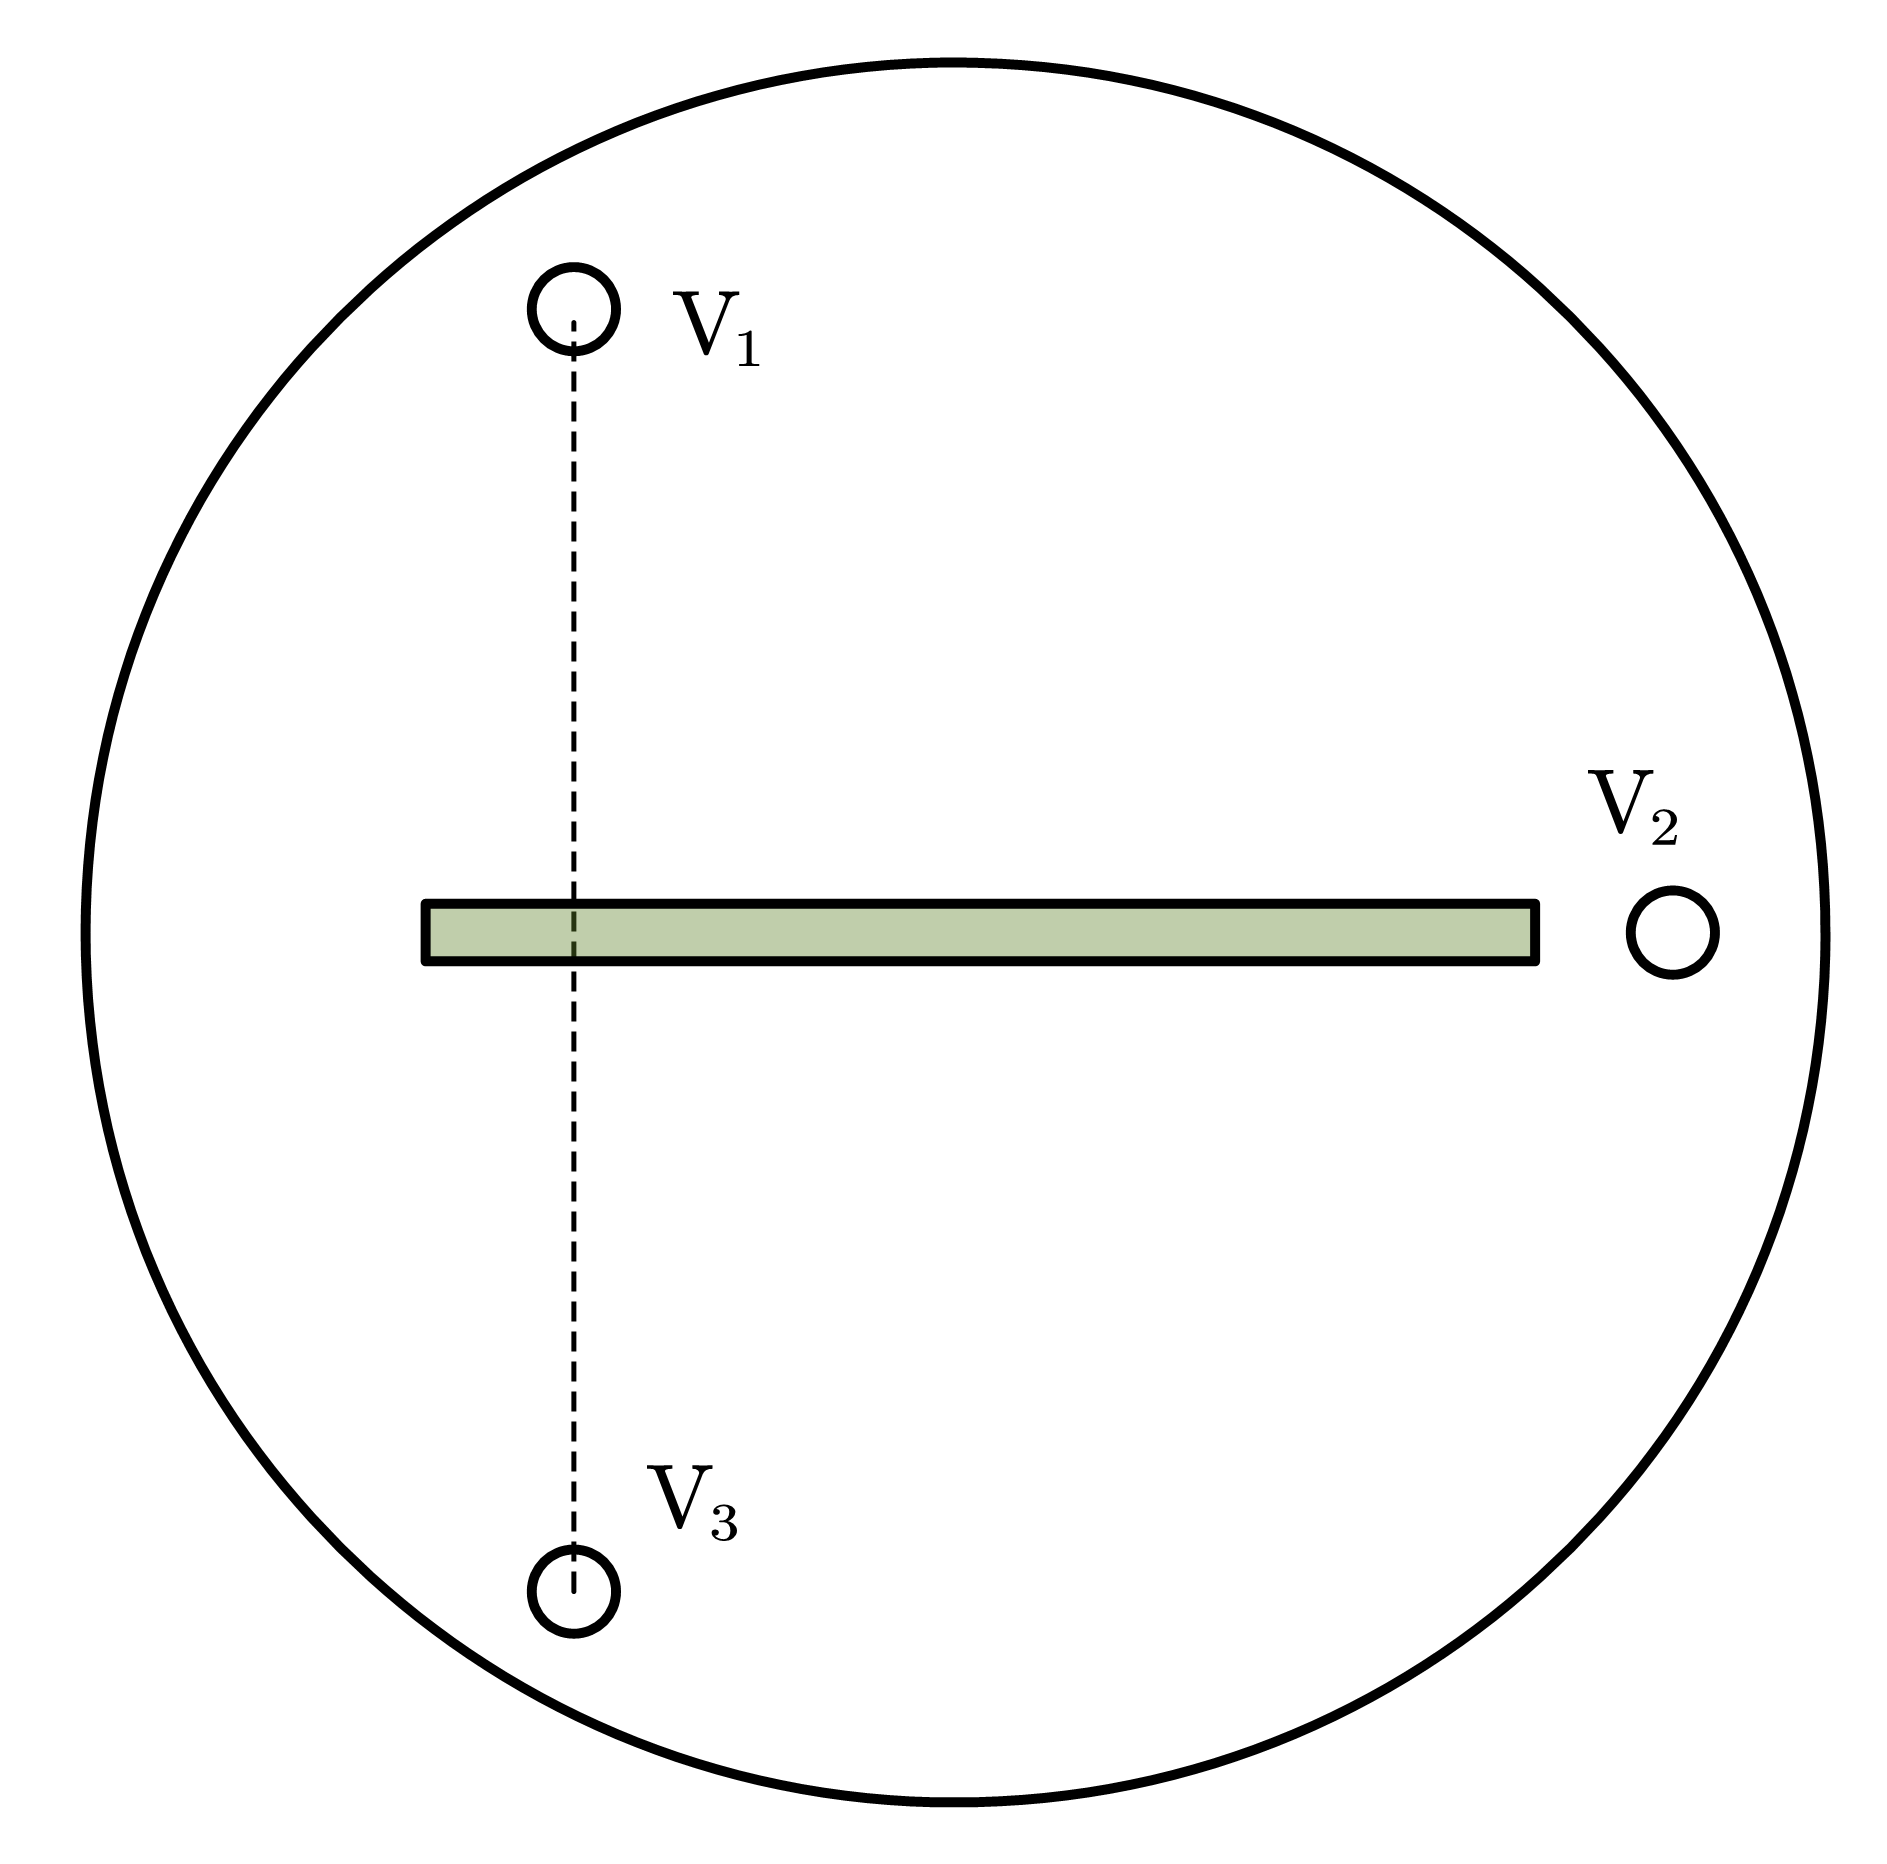
\includegraphics[width=0.3\textwidth]{光栅位置}
	\caption{光栅在在舞台上的位置}
\end{figure}
\clearpage
将光栅按图1所示的方式放置在载物台上。光栅平面与$V_1,V_3$的连线垂直。用汞灯照亮狭缝,使望远镜的叉丝对准狭缝像。这样望远镜的光轴与平行光管的光轴共线。将游标盘与载物台锁定在一起,转动载物台,找到平面光栅反射回来的叉丝像,调节$V_1,V_3$使叉丝像与叉丝重合,随即锁住游标盘,并保持$V_1,V_3$不动。这时就达到了光栅与入射的平行光垂直的要求。此时转动望远镜观察位于零级谱两侧的一级或二级谱线,调节$V_2$和稍微旋转狭缝,使两侧谱线均与叉丝的中心横线垂直,并且上下对称。这时光栅就已经调节好了。
\subsubsection*{误差来源及解决办法}
\par 实验所用的透射光栅是做在一个全息干板上,全息干版的两个面不可能完全平行,因此无论怎样都不可能让入射光线完全垂直与光栅表面。在斜入射的情况下,光栅法线两侧同一级光谱的衍射角分别为
$$
\left.\begin{array}{l}
	\sin \varphi-\sin \theta_{-}=-\dfrac{k \lambda}{d} \\
	\sin \varphi+\sin \theta_{+}=\dfrac{k \lambda}{d}
\end{array}\right\}
$$
\par 两式相减,并考虑$|\theta_{+}-\theta_{-}|=\varphi$
\[\sin{\frac{\theta_{+}-\theta_{-}}{2}}\cos{\frac{\varphi}{2}}=\frac{k \lambda}{d}\]
\par 当$\varphi$很小的时,$\sin{\dfrac{\theta_{+}-\theta_{-}}{2}}=\dfrac{k \lambda}{d}$
\subsubsection*{测量数据}
\par 利用汞光谱线中绿线$\lambda - 546.1\quad nm$的$\pm 1,\pm 2$级光谱之间的夹角$2\theta_1,2\theta_2$,分别求出两个光栅常量。
\subsection*{[数据处理]}
% Please add the following required packages to your document preamble:
% \usepackage{multirow}
% Please add the following required packages to your document preamble:
% \usepackage{multirow}
\par 根据公式$\sin{\dfrac{\theta_{+}-\theta_{-}}{2}}=\dfrac{k \lambda}{d}$计算得:
\begin{table}[!htbp]
	\centering
	\begin{tabular}{c|c|ccc|c|c|c}
		\hline
		\multirow{2}{*}{波长}    & \multirow{2}{*}{级数} & \multicolumn{3}{c|}{衍射角位置}                                   & \multirow{2}{*}{角度} & \multirow{2}{*}{无偏心角度}  & \multirow{2}{*}{光栅常量} \\ \cline{3-5}
		&                     & \multicolumn{1}{c|}{游标号} & \multicolumn{1}{c|}{+k级}    & -k级     &                     &                         &                       \\ \hline
		\multirow{4}{*}{546.1 nm} & \multirow{2}{*}{1}  & \multicolumn{1}{c|}{1}   & \multicolumn{1}{c|}{$9^{\circ}25^{\prime}$} & $9^{\circ}5^{\prime}$   & $19^{\circ}15^{\prime}$               & \multirow{2}{*}{$19^{\circ}025^{\prime}$} & \multirow{2}{*}{3301nm}     \\ \cline{3-6}
		&                     & \multicolumn{1}{c|}{2}   & \multicolumn{1}{c|}{$9^{\circ}29^{\prime}$} & $9^{\circ}21^{\prime}$  & $18^{\circ}50^{\prime}$                &                         &                       \\ \cline{2-8} 
		& \multirow{2}{*}{2}  & \multicolumn{1}{c|}{1}   & \multicolumn{1}{c|}{$19^{\circ}10^{\prime}$} & $20^{\circ}01^{\prime}$ & $39^{\circ}11^{\prime}$               & \multirow{2}{*}{$39^{\circ}205^{\prime}$} & \multirow{2}{*}{3245nm}     \\ \cline{3-6}
		&                     & \multicolumn{1}{c|}{2}   & \multicolumn{1}{c|}{$19^{\circ}30^{\prime}$} & $20^{\circ}00^{\prime}$    & $39^{\circ}30^{\prime}$                &                         &                       \\ \hline
	\end{tabular}	
\end{table}
\par 所以$\overline{d}=3273nm$
\clearpage
% Please add the following required packages to your document preamble:
% \usepackage{multirow}
\begin{table}[!htbp]
	\centering
	\begin{tabular}{c|c|ccc|c|c|c}
		\hline
		\multirow{2}{*}{汞黄线} & \multirow{2}{*}{级数} & \multicolumn{3}{c|}{衍射角位置}                                                                        & \multirow{2}{*}{角度}     & \multirow{2}{*}{无偏心角度}                   & \multirow{2}{*}{波长} \\ 
		\cline{3-5}
		&                     & \multicolumn{1}{c|}{游标号} & \multicolumn{1}{c|}{k}                       & k                       &                         &                                          &                       \\ 
		\hline
		\multirow{2}{*}{黄1}  & \multirow{2}{*}{2}  & \multicolumn{1}{c|}{1}   & \multicolumn{1}{c|}{$20^{\circ}08^{\prime}$} & $20^{\circ}50^{\prime}$ & $40^{\circ}58^{\prime}$ & \multirow{2}{*}{$40^{\circ}48^{\prime}$} & \multirow{2}{*}{570.5nm}     \\ 
		\cline{3-6}
		&                     & \multicolumn{1}{c|}{2}   & \multicolumn{1}{c|}{$19^{\circ}52^{\prime}$} & $20^{\circ}40^{\prime}$ & $40^{\circ}38^{\prime}$ &                                          &                       \\ 
		\hline
		\multirow{2}{*}{黄2}  & \multirow{2}{*}{2}  & \multicolumn{1}{c|}{1}   & \multicolumn{1}{c|}{$20^{\circ}15^{\prime}$} & $20^{\circ}40^{\prime}$ & $40^{\circ}55^{\prime}$ & \multirow{2}{*}{$40^{\circ}58^{\prime}$} & \multirow{2}{*}{572.7nm}     \\ 
		\cline{3-6}
		&                     & \multicolumn{1}{c|}{2}   & \multicolumn{1}{c|}{$20^{\circ}11^{\prime}$} & $20^{\circ}50^{\prime}$ & $41^{\circ}01^{\prime}$ &                                          &                       \\ 
		\hline
	\end{tabular}
\end{table}
\par 跟标准值$\lambda_1 = 577.0nm,\lambda_2 = 579.1nm$计算得到误差为:
\[ \Delta \lambda_1 = \frac{|577.0-570.5|}{577.0}=0.011  \]
\[\Delta \lambda_1 = \frac{|579.1-572.7|}{579.1}=0.011\]
\par 而角色散
\[D = \frac{\Delta \varphi}{2.1nm} = \frac{10^{\prime}}{2.1nm} = 1385 rad/m = 1.385 \mu rad / nm\]

\end{document}
